In dis chapter we go tha fuck into detail bout how tha fuck tha DSMC model is implemented up in C{}\verb!++!. We assume dat tha reader is familiar wit tha programmin language. Instead of goin all up in all tha classes n' they relations, we follow tha time line of a simulation, goin from tha initialization of tha system ta how tha fuck tha timestep is computed. Y'all KNOW dat shit, muthafucka! This type'a shiznit happens all tha time. For convenience, a UML diagram is shown up in figure \ref{fig:dsmc_uml_diagram}.
\begin{figure}[h]
\begin{center}
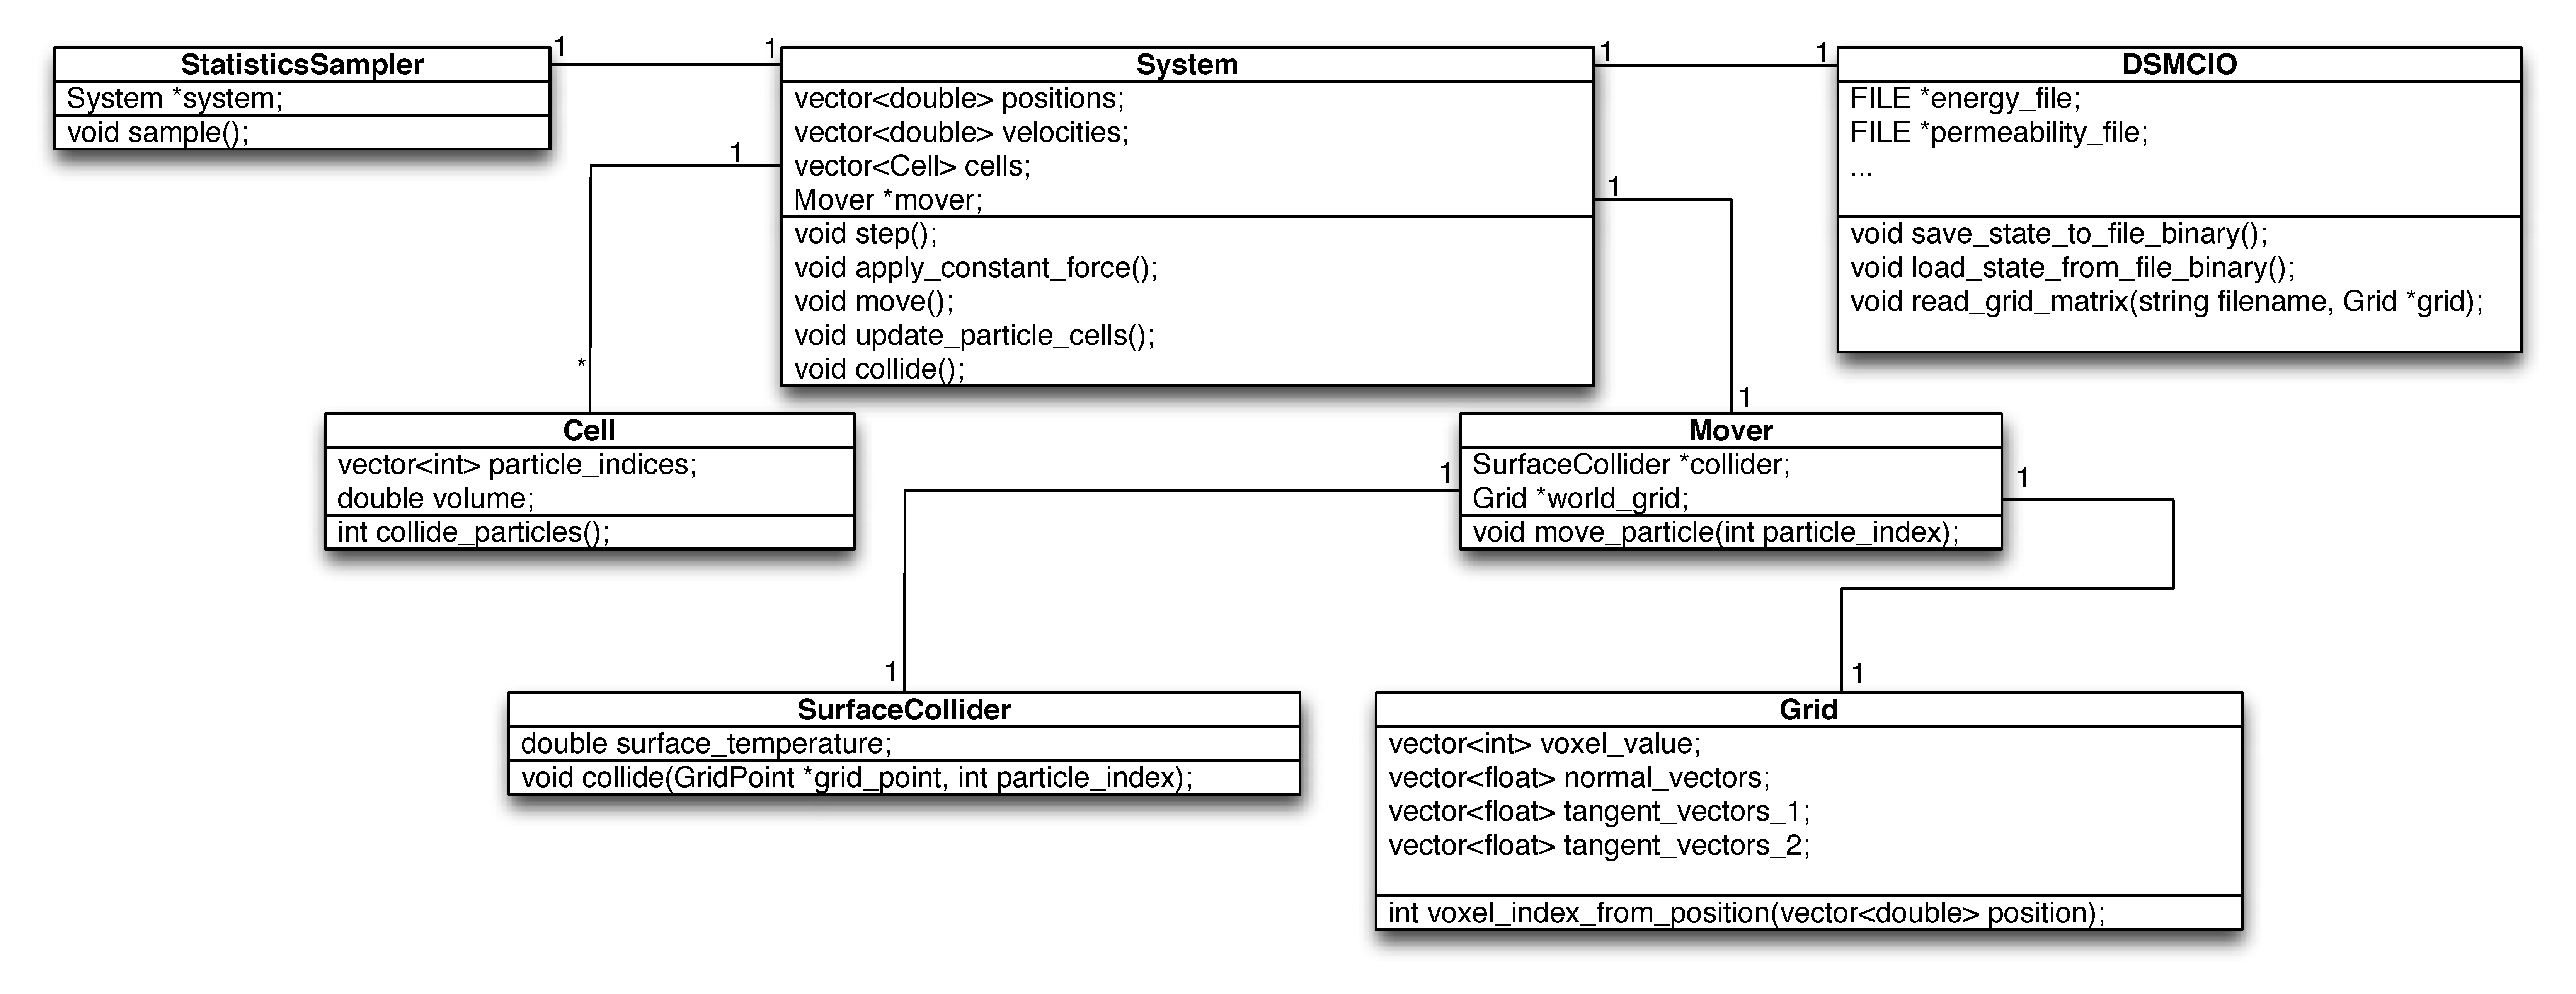
\includegraphics[width=0.9\textwidth, trim=0cm 0cm 0cm 0cm, clip]{DSMC/figures/dsmcuml.eps}
\end{center}
\caption{A UML-diagram showin how tha fuck tha classes up in tha DSMC program is related ta each other.}
\label{fig:dsmc_uml_diagram}
\end{figure}
\\
Da first step of tha full program is ta create tha geometry we want tha particlez ta be confined by. We explain how tha fuck dat is done up in section \ref{sec:dsmc_complex_geometries}. Then, we can initialize a system by addin particlez randomly inside tha geometry. Their velocitizzles should be Maxwell-Boltzmann distributed, as busted lyrics bout up in section \ref{eq:maxwell_boltzmann_vector_probability}. Da initialization process is explained up in section \ref{sec:dsmc_implementation_initialization} before we is locked n loaded ta big-ass up tha timesteps fo' realz. A timestep is divided tha fuck into four stages. These stages are
\begin{itemize}
    \item accelerate particlez ta induce flow,
    \item move particlez n' big-ass up surface interactions,
    \item update collision cells,
    \item big-ass up collisions between particles,
\end{itemize}
which all is discussed up in section \ref{sec:dsmc_implementation_timestep}. This is every last muthafuckin thang we need ta run a DSMC program up in \textit{any} geometry we want. Da only thang left ta explain is how tha fuck our crazy asses have parallelized tha code, allowin it ta run on nuff processors on a supercomputer n' shit. This final piece is explained up in section \ref{sec:dmsc_parallelization}. Da full code be available, on demand, by contactin tha lyricist at \url{anderhaf@fys.uio.no}.